\documentclass[12pt]{article}
\usepackage{times}
\usepackage{graphicx} % Required for inserting images
\usepackage[margin=1in]{geometry} % Adjust margins to 1 inch
\usepackage{float} % Required for the [H] float option

\title{2XC3-Final-Project}
\author{Joshua Finemore, Austin Bray, Neel Oza}
\date{March 2025}

\begin{document}

\maketitle
\tableofcontents 

\section*{Notes}
\addcontentsline{toc}{section}{Notes}
Some of the questions in the assignment tell us to label a section with a specific title but we named them based on the question. For example, Part 6 says to discuss points in a section labelled "Part 4" but it is under a section "Part 6: Organize your code as per UML diagram" as this is a more descriptive section name.

\newpage
\section*{Part 1: Create a Team Charter}
\addcontentsline{toc}{section}{Part 1: Create a Team Charter}

\subsection*{Communication Protocol}
\addcontentsline{toc}{subsection}{Communication Protocol}
Our group will use Discord and a reasonable timeline for a response in around 2-3 hours.

\subsection*{Penalty for failure to adhere to communication protocol}
\addcontentsline{toc}{subsection}{Penalty for failure to adhere to communication protocol}
If a group member fails to follow the communication protocol in multiple instances, then they will be reported to the TAs, and punished to the full extent of McMaster Policy.

\subsection*{Collaboration Software}
\addcontentsline{toc}{subsection}{Collaboration Software}
Our group will use GitHub to collaborate and version control our code. In instances where synchronous development is required, we will communicate over Discord or meet up in person.

\subsection*{Resolving Team Disputes}
\addcontentsline{toc}{subsection}{Resolving Team Disputes}
If two group members have a dispute, the third will vote on who is right. The member deemed to be in the wrong gets one strike towards the violation of communication protocol.

\newpage
\section*{Part 2: Single source shortest path algorithms}
\addcontentsline{toc}{section}{Part 2: Single source shortest path algorithms}

For the experiments we ran 100 trials with 100 random graphs in each trial. We also ran 4 different experiments with varying densities. This will allow for a better comparison between the two algorithms when they have low and high densities. For all the experiments we used $k=num\_of\_nodes-1$ so that we are comparing the full functionality of the algorithms. \newline
\newline
The results from the experiments show us that Bellman-Ford is slower than Dijkstra's for dense graphs. We know that Bellman-Ford should also be slower than Dijkstra's, since Dijkstra's is $O(E \cdot log(V))$ and Bellman-Ford is $O(V\cdot E)$. Although our experiments show that Bellman-Ford is faster than Dijkstra's for sparse graphs. The reasoning for this is due to Dijkstra's being implemented with a indexed heap priority queue that uses python code for reducing a key resulting in slower execution, while Bellman-Ford is implemented using a queue and inbuilt python functions which actually run in C therefore speeding up the execution.

\subsection*{2.1: Dijkstra's Algorithm}
\addcontentsline{toc}{subsection}{2.1: Dijkstra's Algorithm}
The implementation for dijkstra's algorithm is heavily based on the implementation from the 2C03 textbook, Algorithms 4th Edition by Robert Sedgewick, Kevin Wayne.

\subsection*{2.2: Bellman-Ford's Algorithm}
\addcontentsline{toc}{subsection}{2.2: Bellman-Ford's Algorithm}
The implementation for bellman-ford's algorithm is heavily based on the implementation from the 2C03 textbook, Algorithms 4th Edition by Robert Sedgewick, Kevin Wayne.

\subsection*{2.3: Experiment with Dijkstra's and Bellman-Ford's Algorithm}
\addcontentsline{toc}{subsection}{2.3: Experiment with Dijkstra's and Bellman-Ford's Algorithm}

\subsubsection*{Bellman-Ford's Algorithm Visualizations}
\addcontentsline{toc}{subsubsection}{Bellman-Ford's Algorithm Visualizations}

\begin{figure}[H]
    \centering
    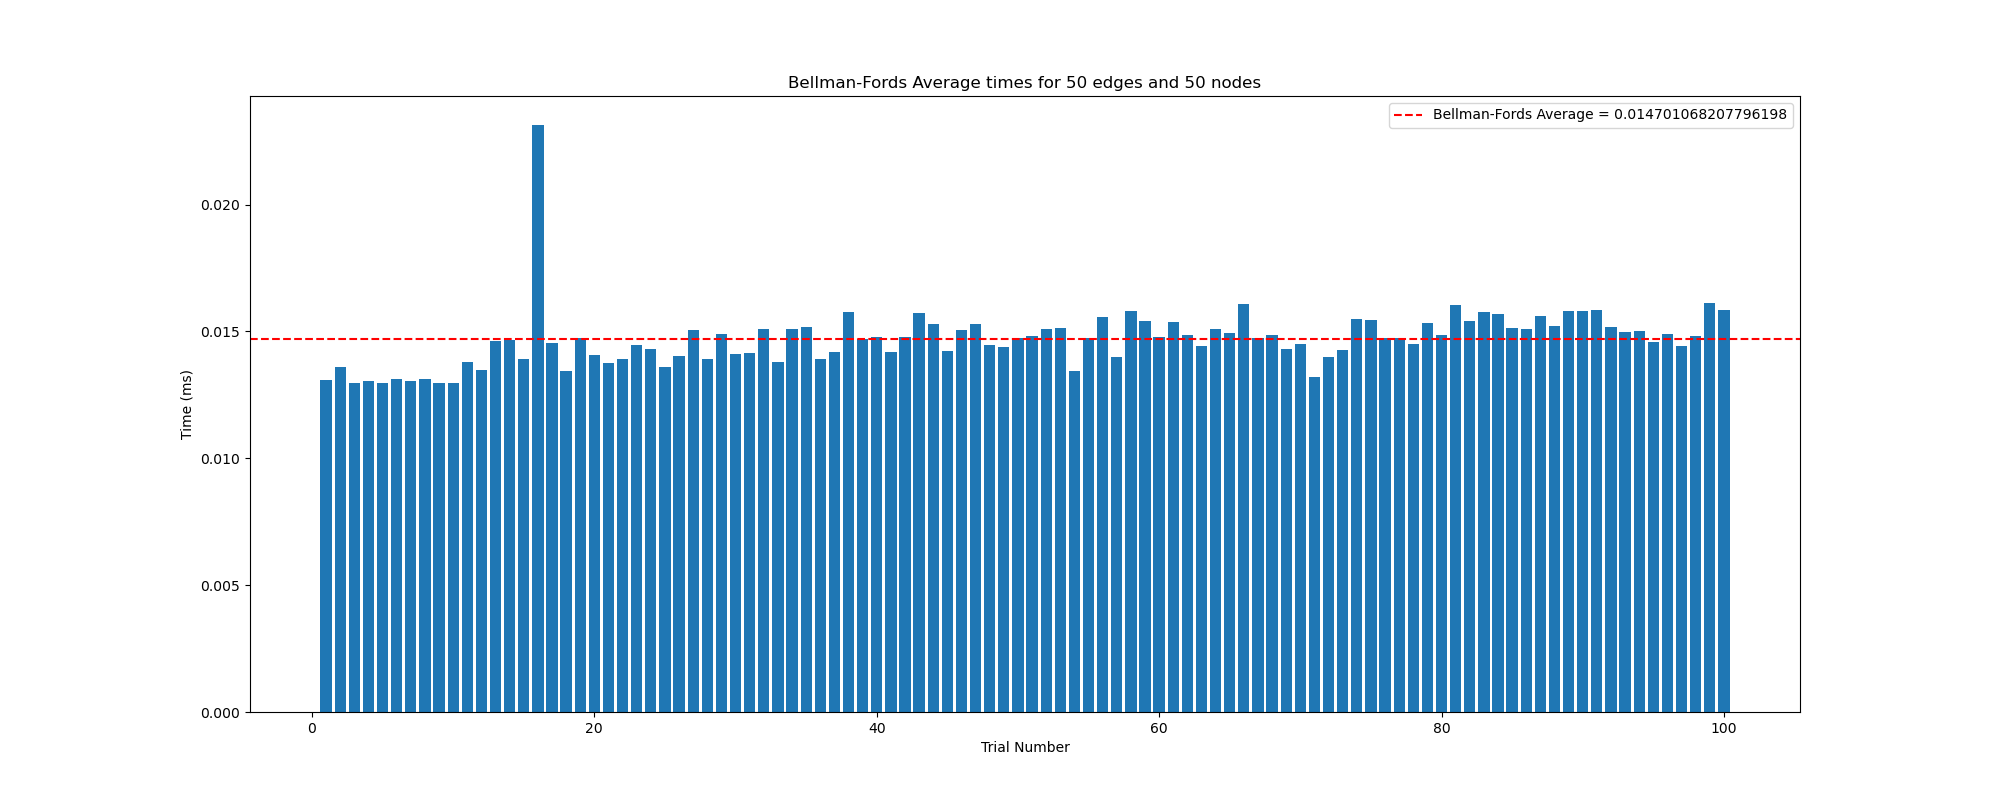
\includegraphics[width=\textwidth]{images/Bellman-Fords Average times for 50 edges and 50 nodes.png}
    \caption{Bellman-Fords Average times for 50 edges and 50 nodes}
\end{figure}

\begin{figure}[H]
    \centering
    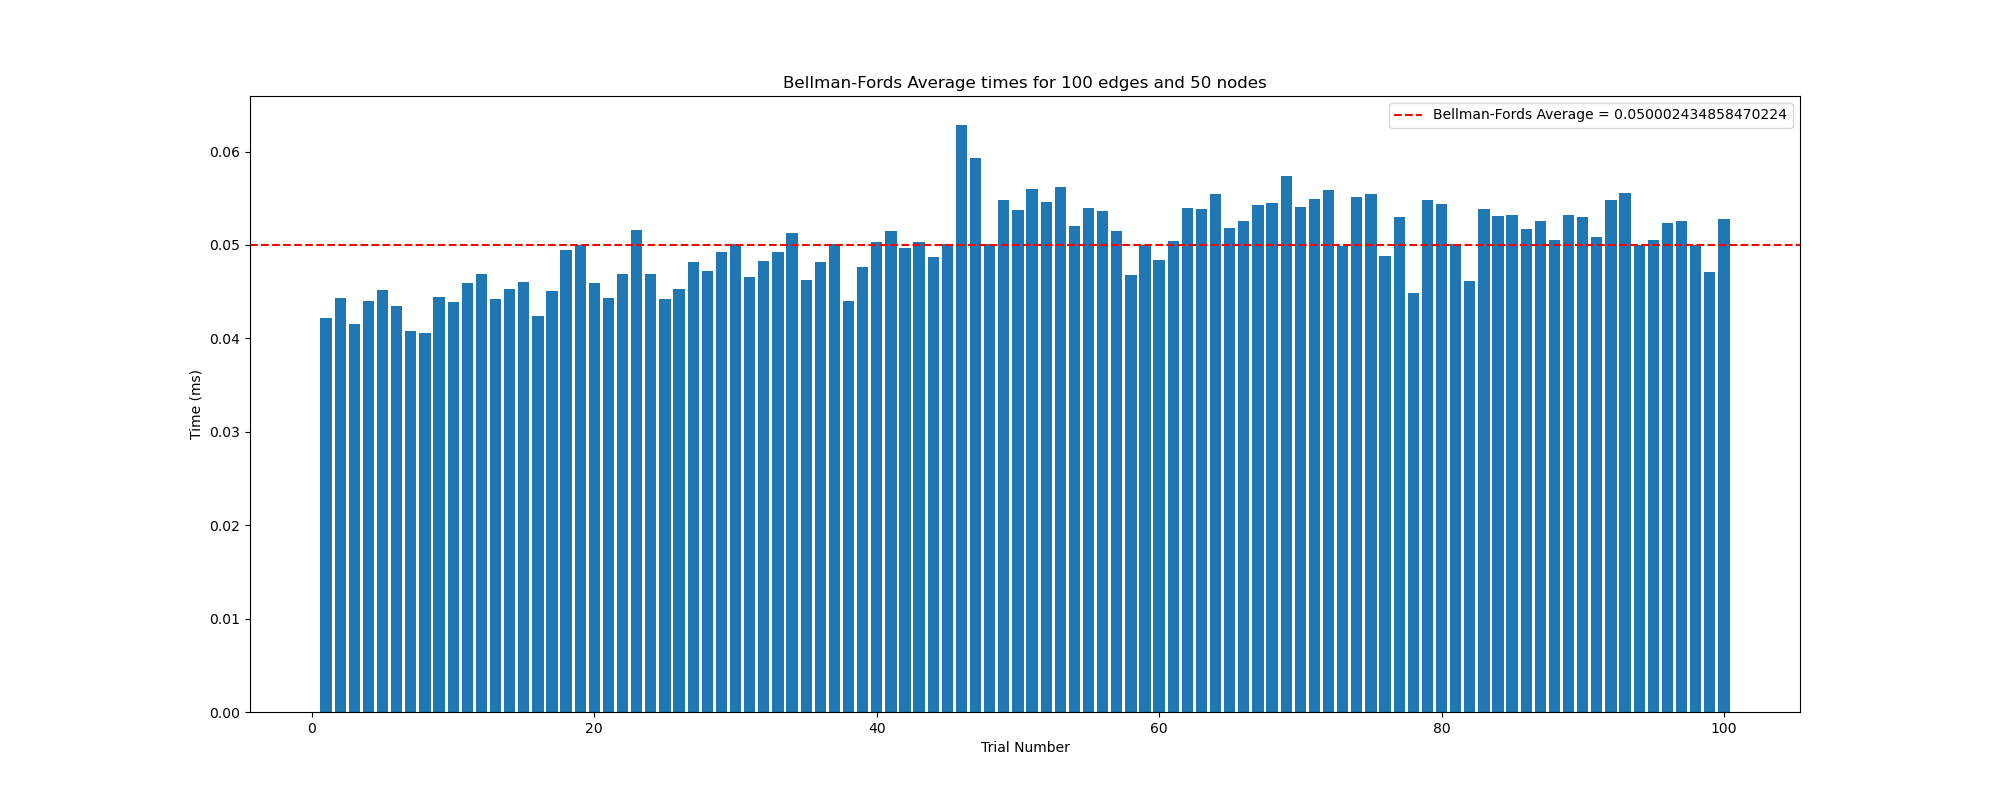
\includegraphics[width=\textwidth]{images/Bellman-Fords Average times for 100 edges and 50 nodes.png}
    \caption{Bellman-Fords Average times for 100 edges and 50 nodes}
\end{figure}

\begin{figure}[H]
    \centering
    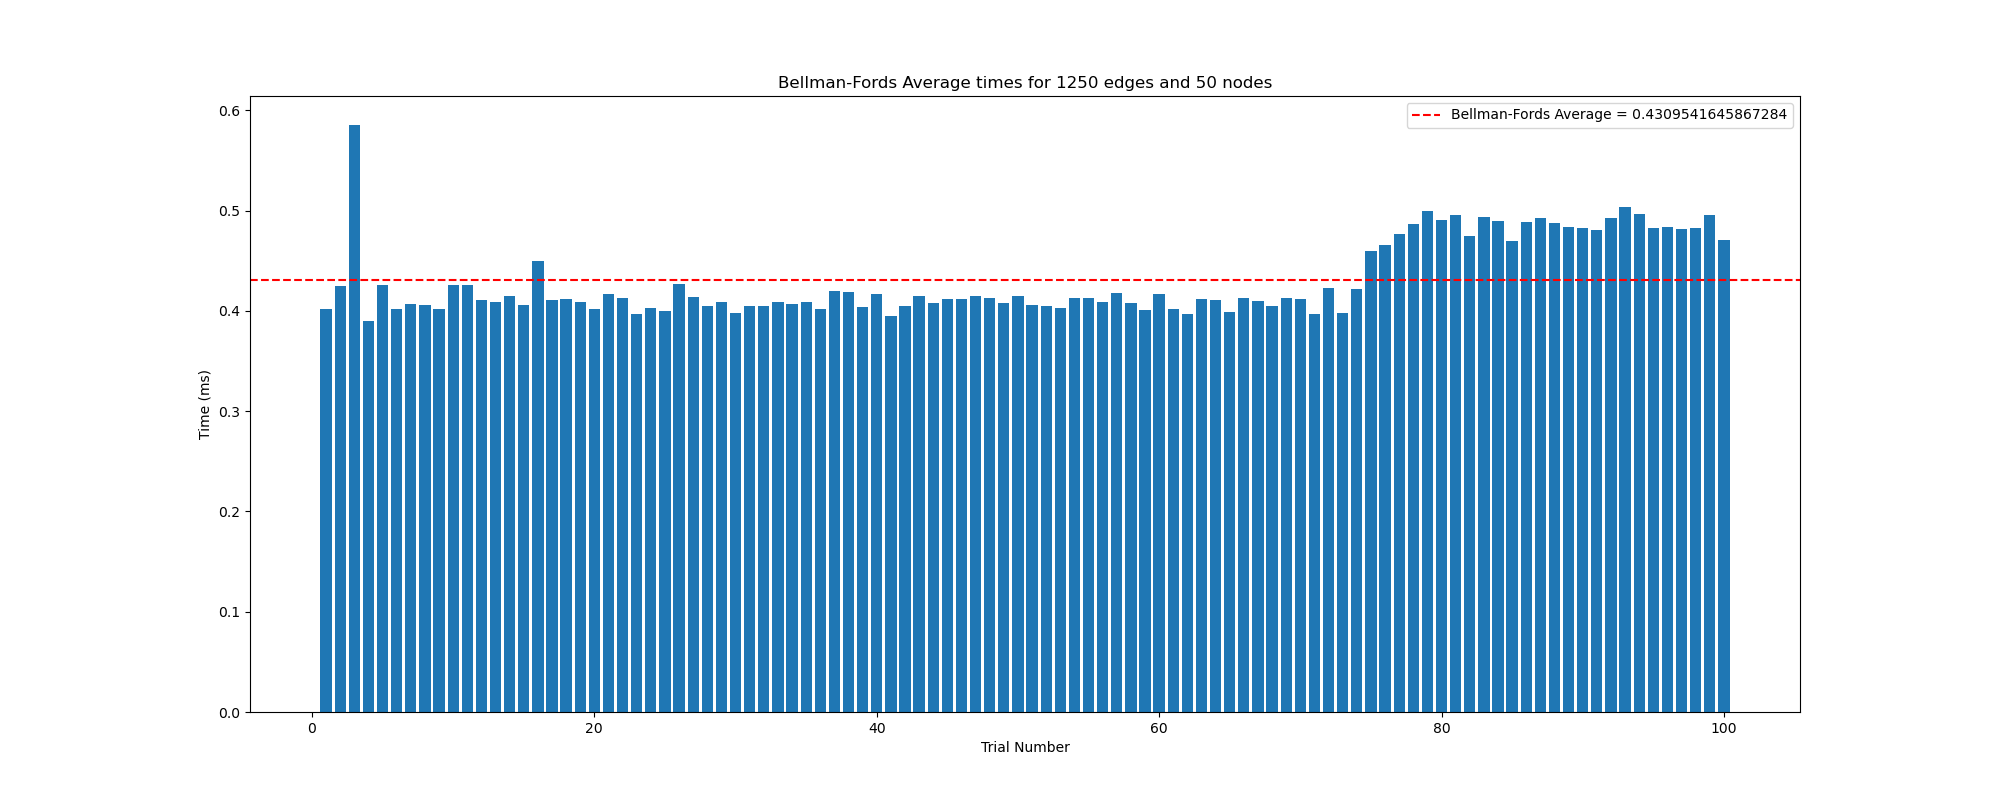
\includegraphics[width=\textwidth]{images/Bellman-Fords Average times for 1250 edges and 50 nodes.png}
    \caption{Bellman-Fords Average times for 1250 edges and 50 nodes}
\end{figure}

\begin{figure}[H]
    \centering
    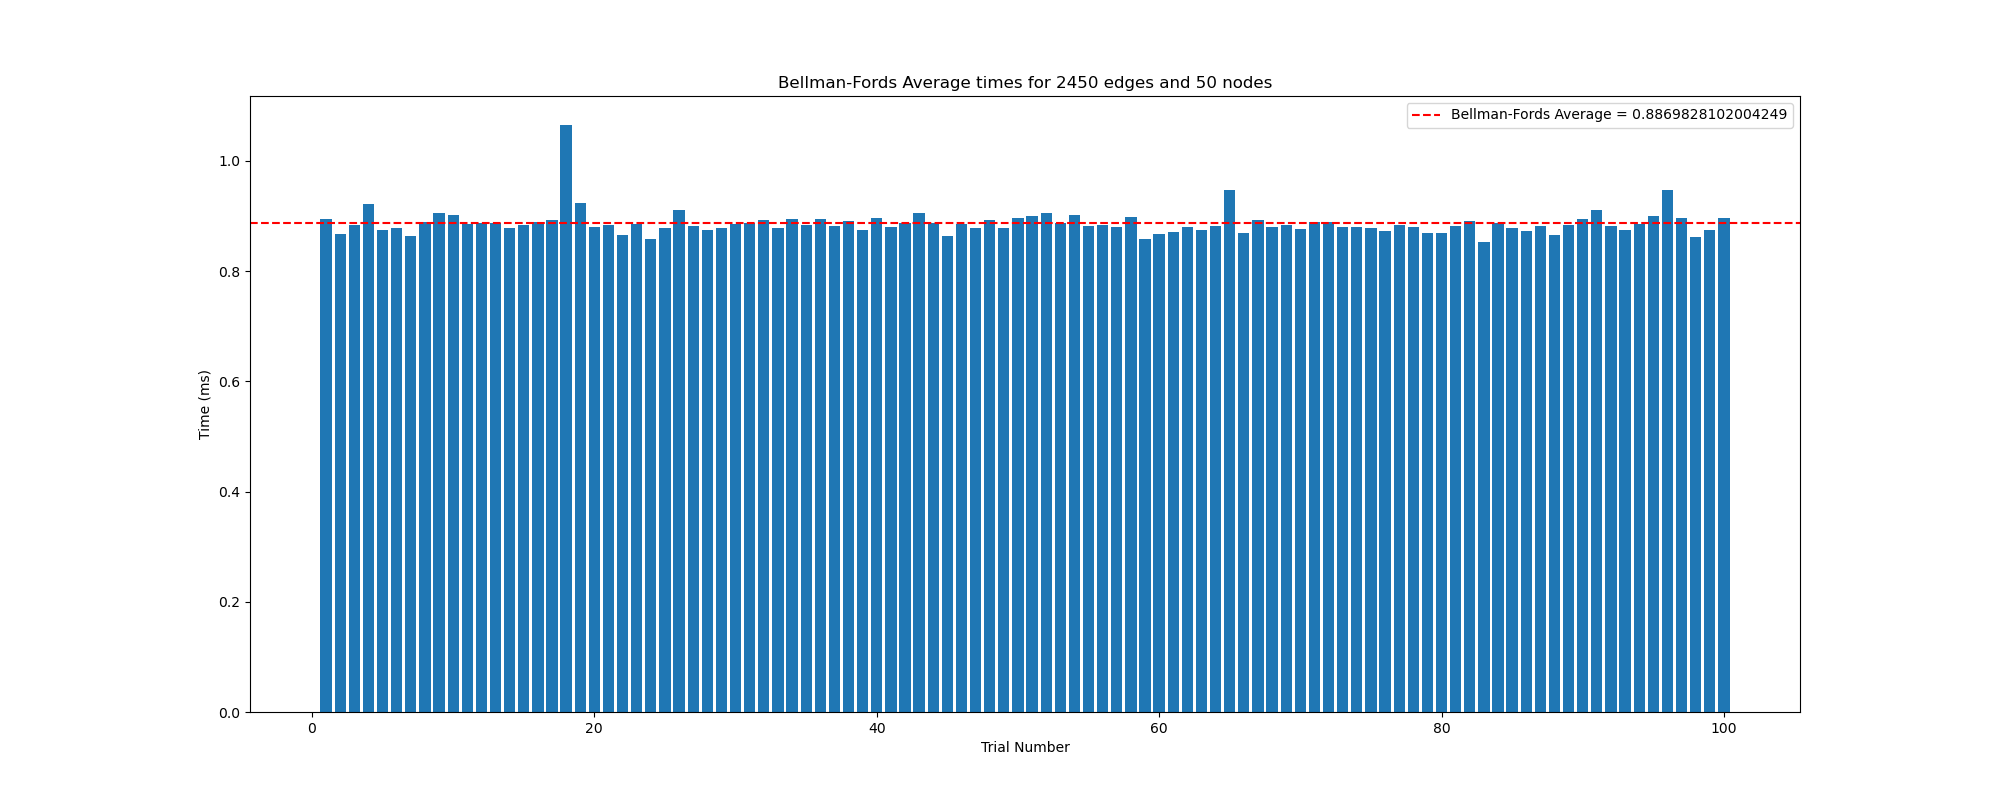
\includegraphics[width=\textwidth]{images/Bellman-Fords Average times for 2450 edges and 50 nodes.png}
    \caption{Bellman-Fords Average times for 2450 edges and 50 nodes}
\end{figure}

\begin{figure}[H]
    \centering
    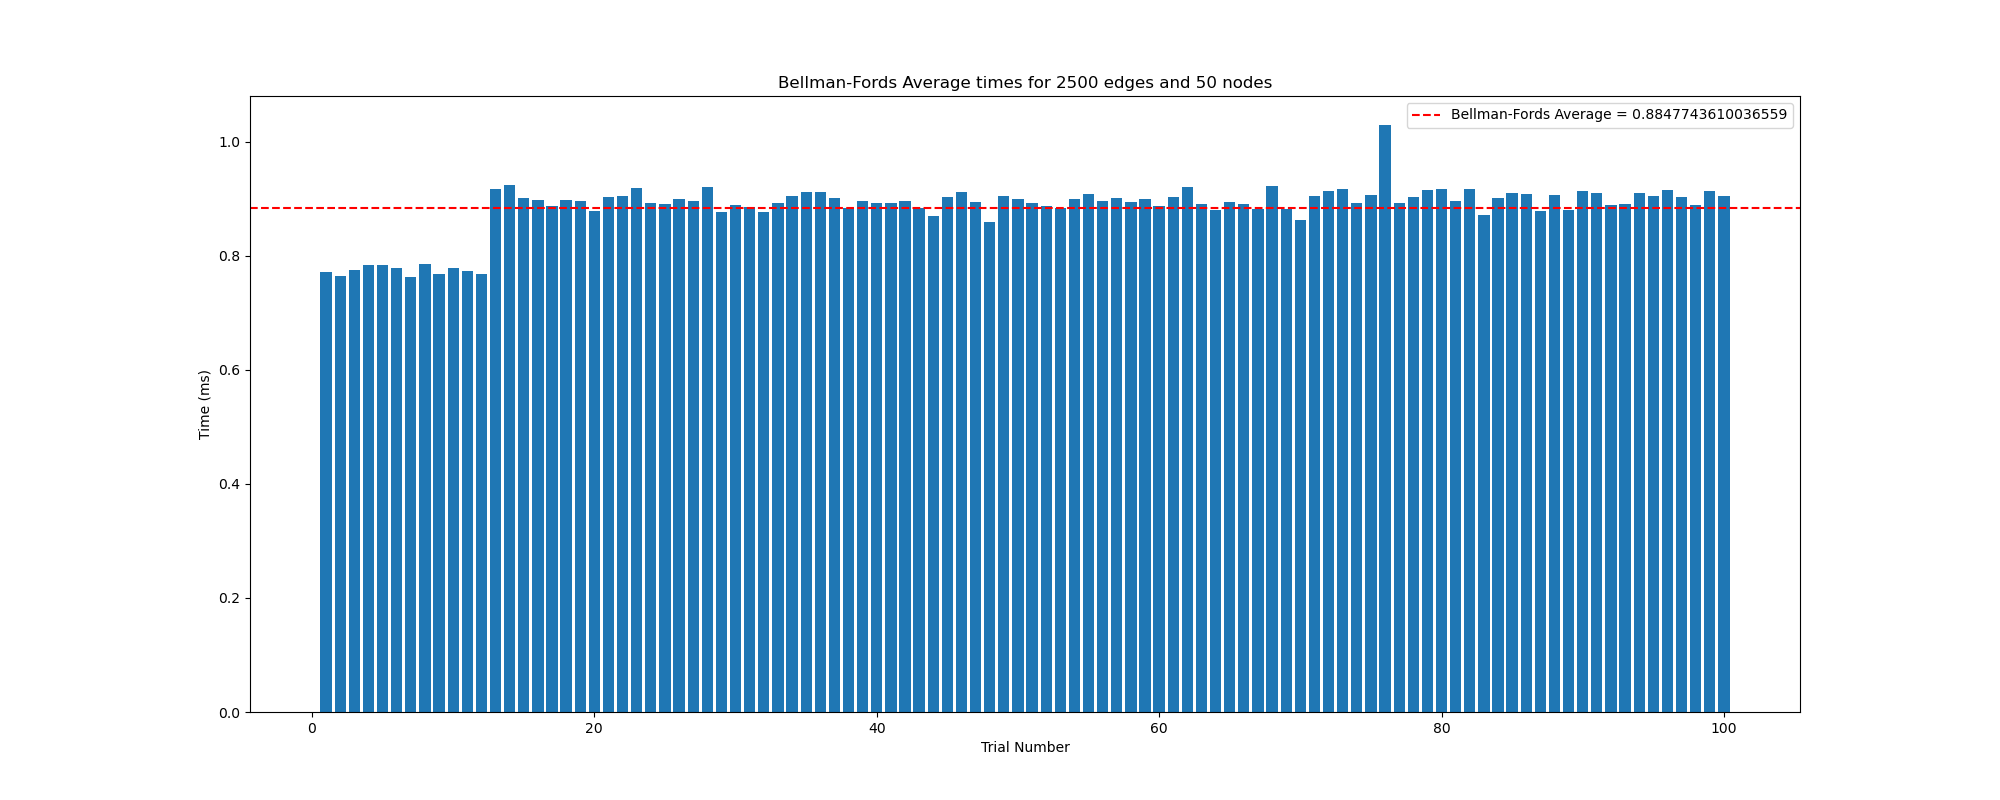
\includegraphics[width=\textwidth]{images/Bellman-Fords Average times for 2500 edges and 50 nodes.png}
    \caption{Bellman-Fords Average times for 2500 edges and 50 nodes}
\end{figure}

\subsubsection*{Dijkstra's Algorithm Visualizations}
\addcontentsline{toc}{subsubsection}{Dijkstra's Algorithm Visualizations}

\begin{figure}[H]
    \centering
    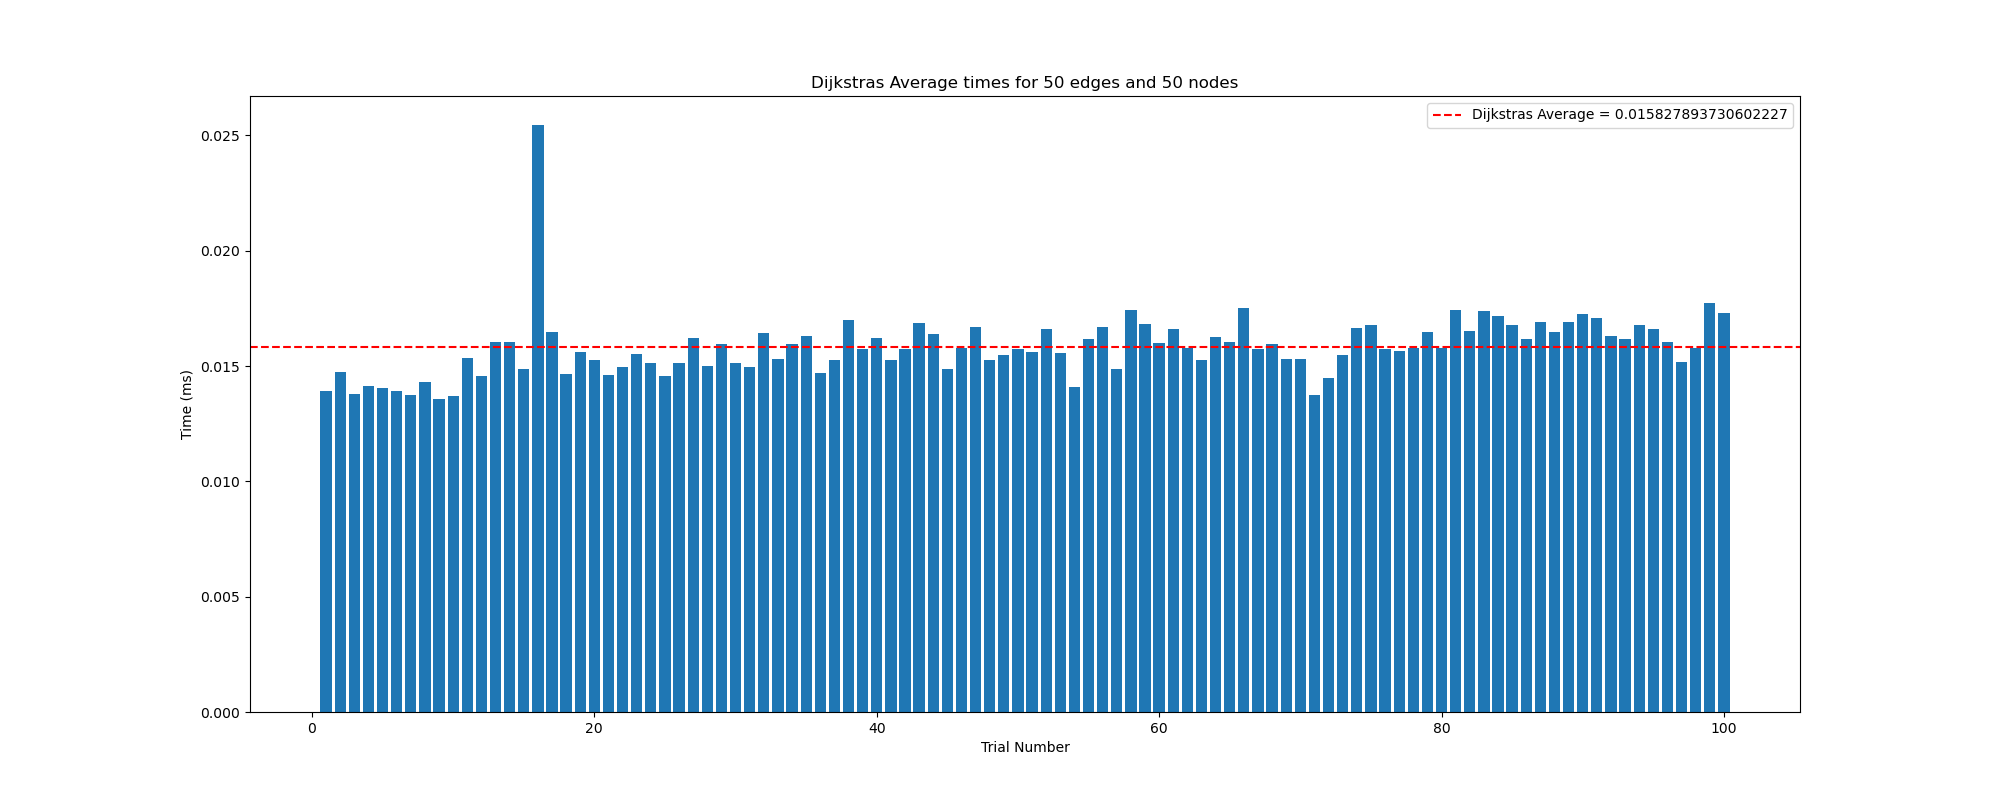
\includegraphics[width=\textwidth]{images/Dijkstras Average times for 50 edges and 50 nodes.png}
    \caption{Dijkstra's Average times for 50 edges and 50 nodes}
\end{figure}

\begin{figure}[H]
    \centering
    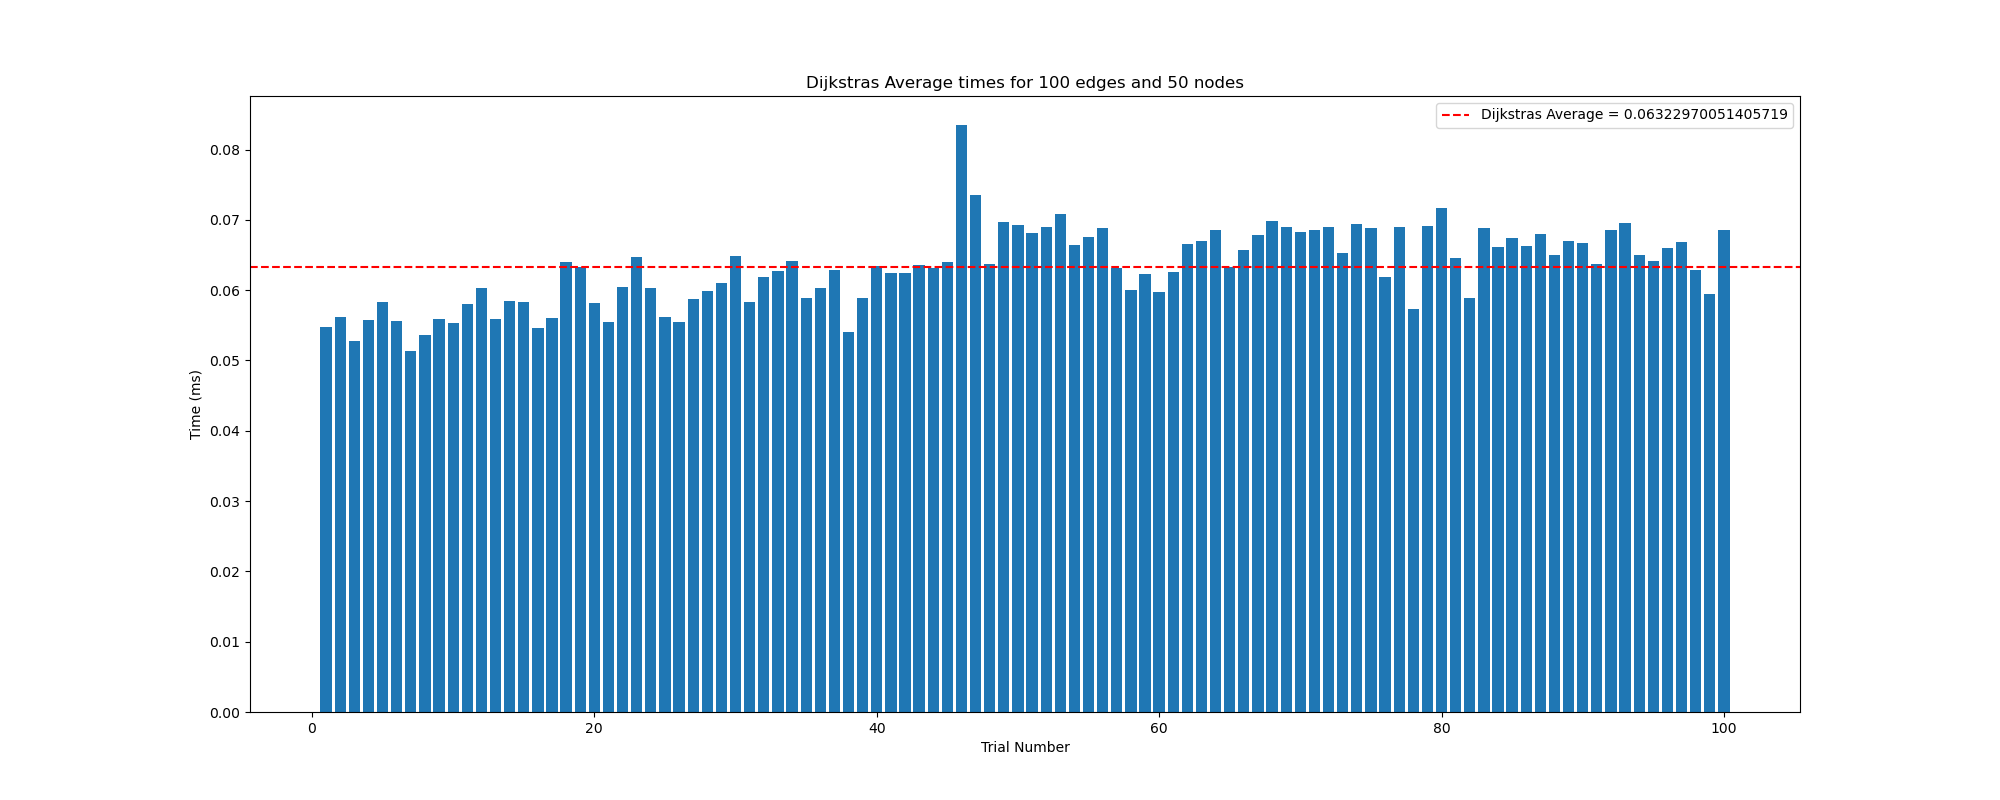
\includegraphics[width=\textwidth]{images/Dijkstras Average times for 100 edges and 50 nodes.png}
    \caption{Dijkstra's Average times for 100 edges and 50 nodes}
\end{figure}

\begin{figure}[H]
    \centering
    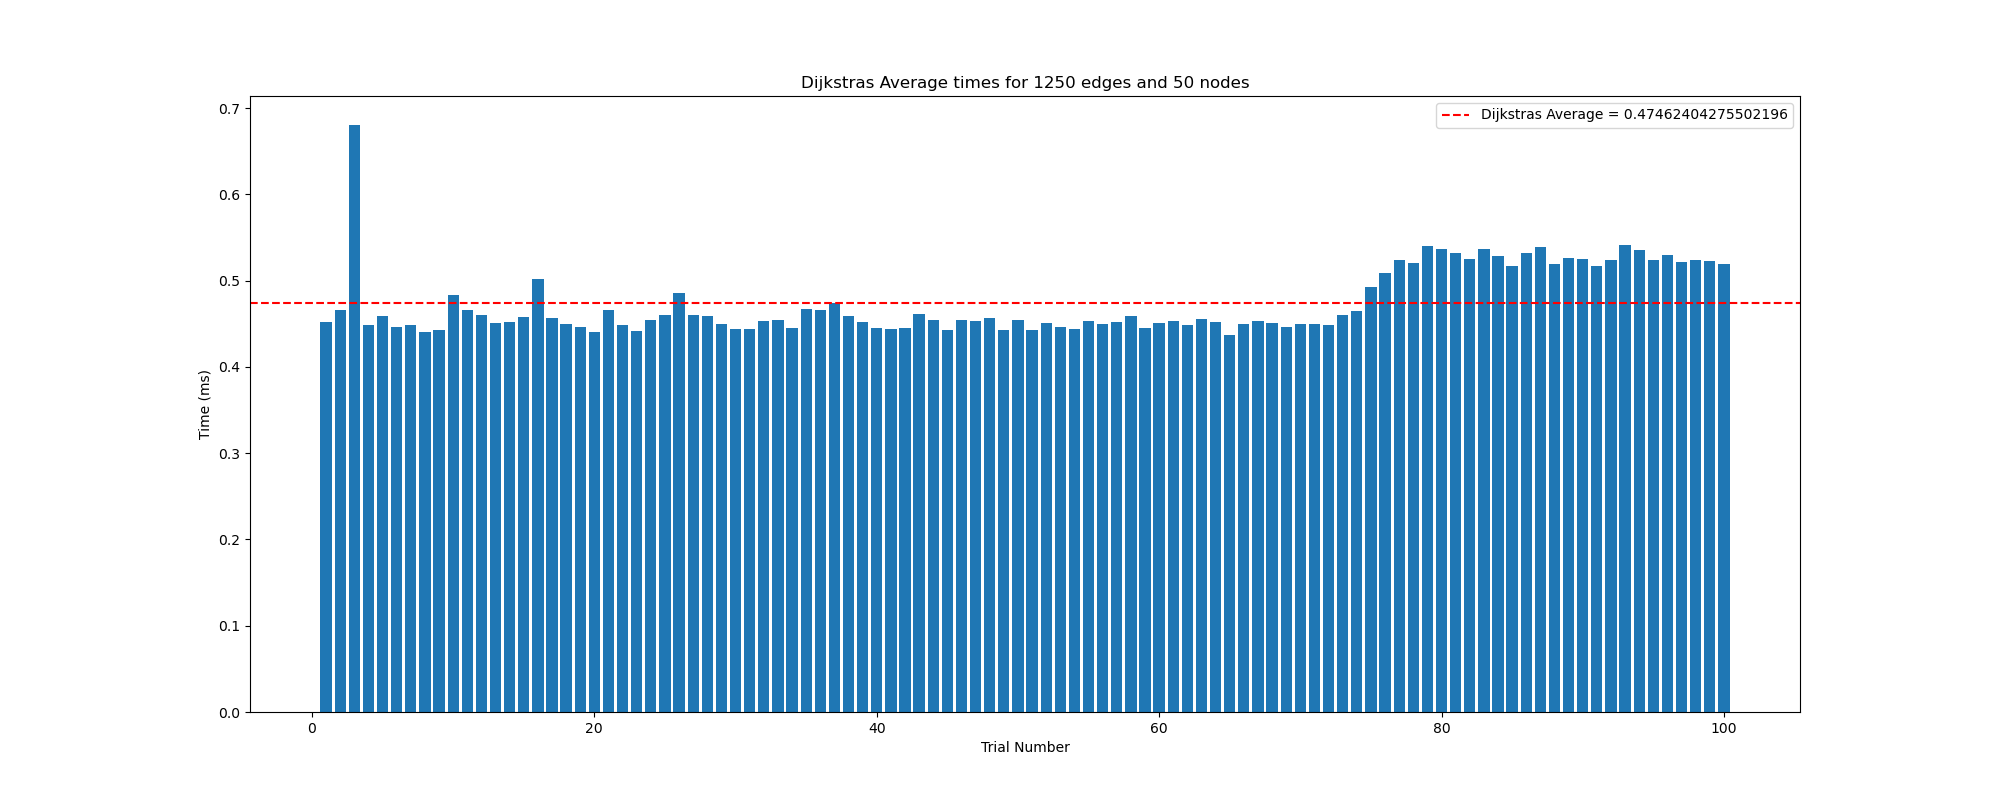
\includegraphics[width=\textwidth]{images/Dijkstras Average times for 1250 edges and 50 nodes.png}
    \caption{Dijkstra's Average times for 1250 edges and 50 nodes}
\end{figure}

\begin{figure}[H]
    \centering
    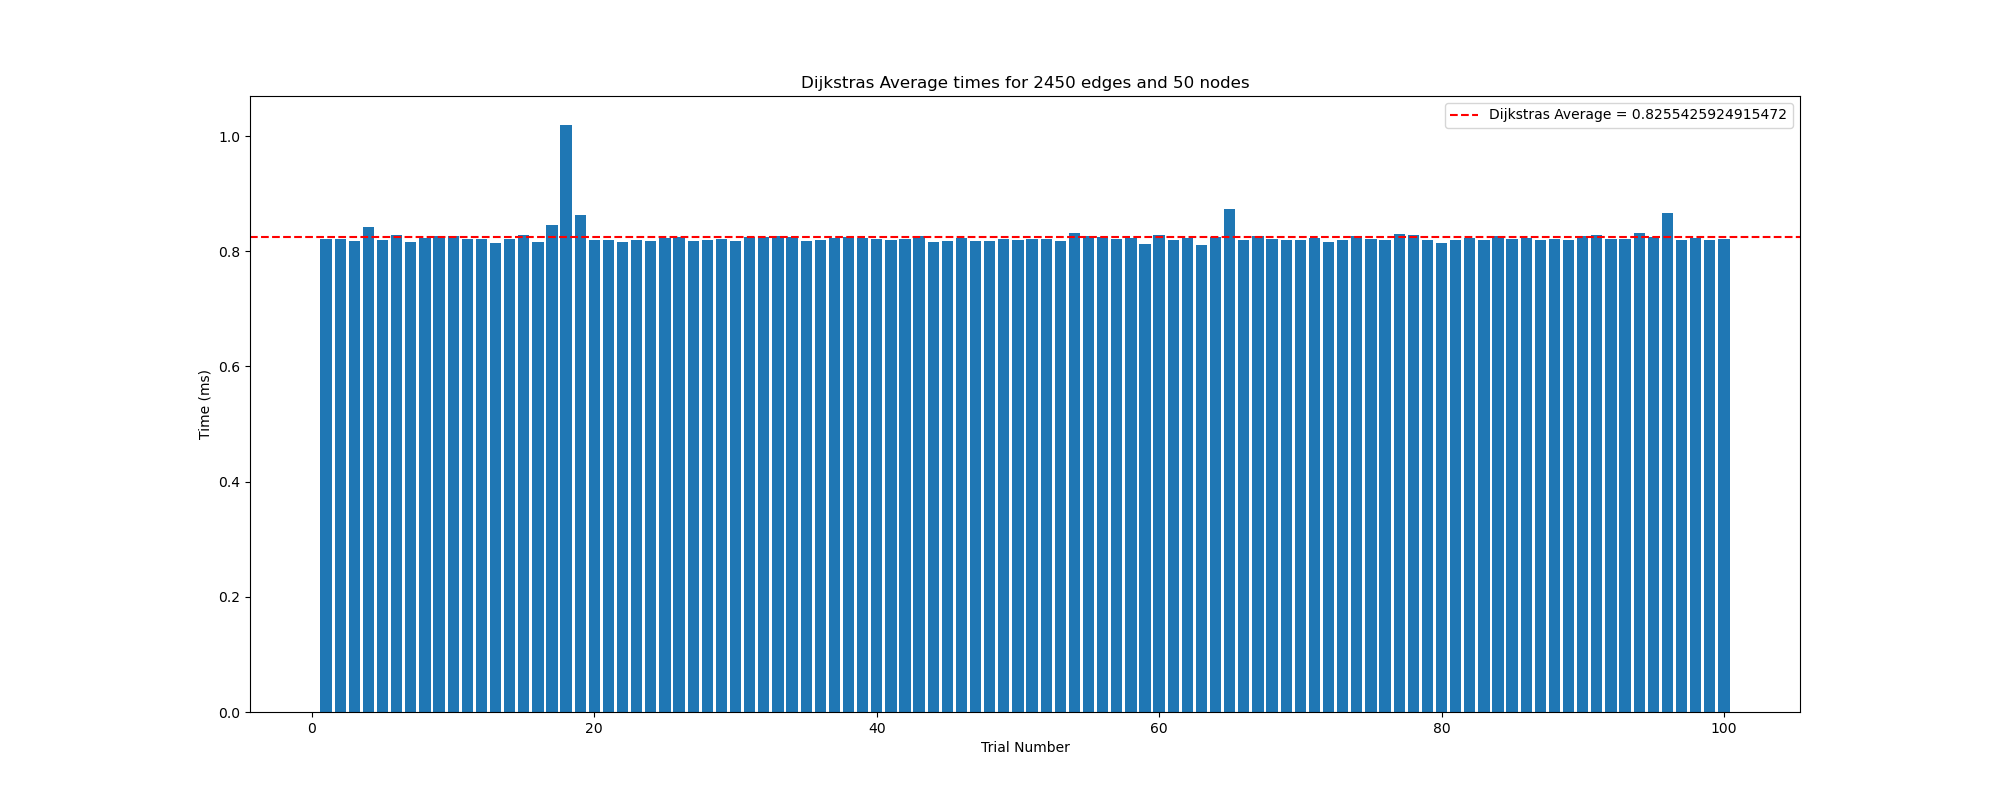
\includegraphics[width=\textwidth]{images/Dijkstras Average times for 2450 edges and 50 nodes.png}
    \caption{Dijkstra's Average times for 2450 edges and 50 nodes}
\end{figure}

\begin{figure}[H]
    \centering
    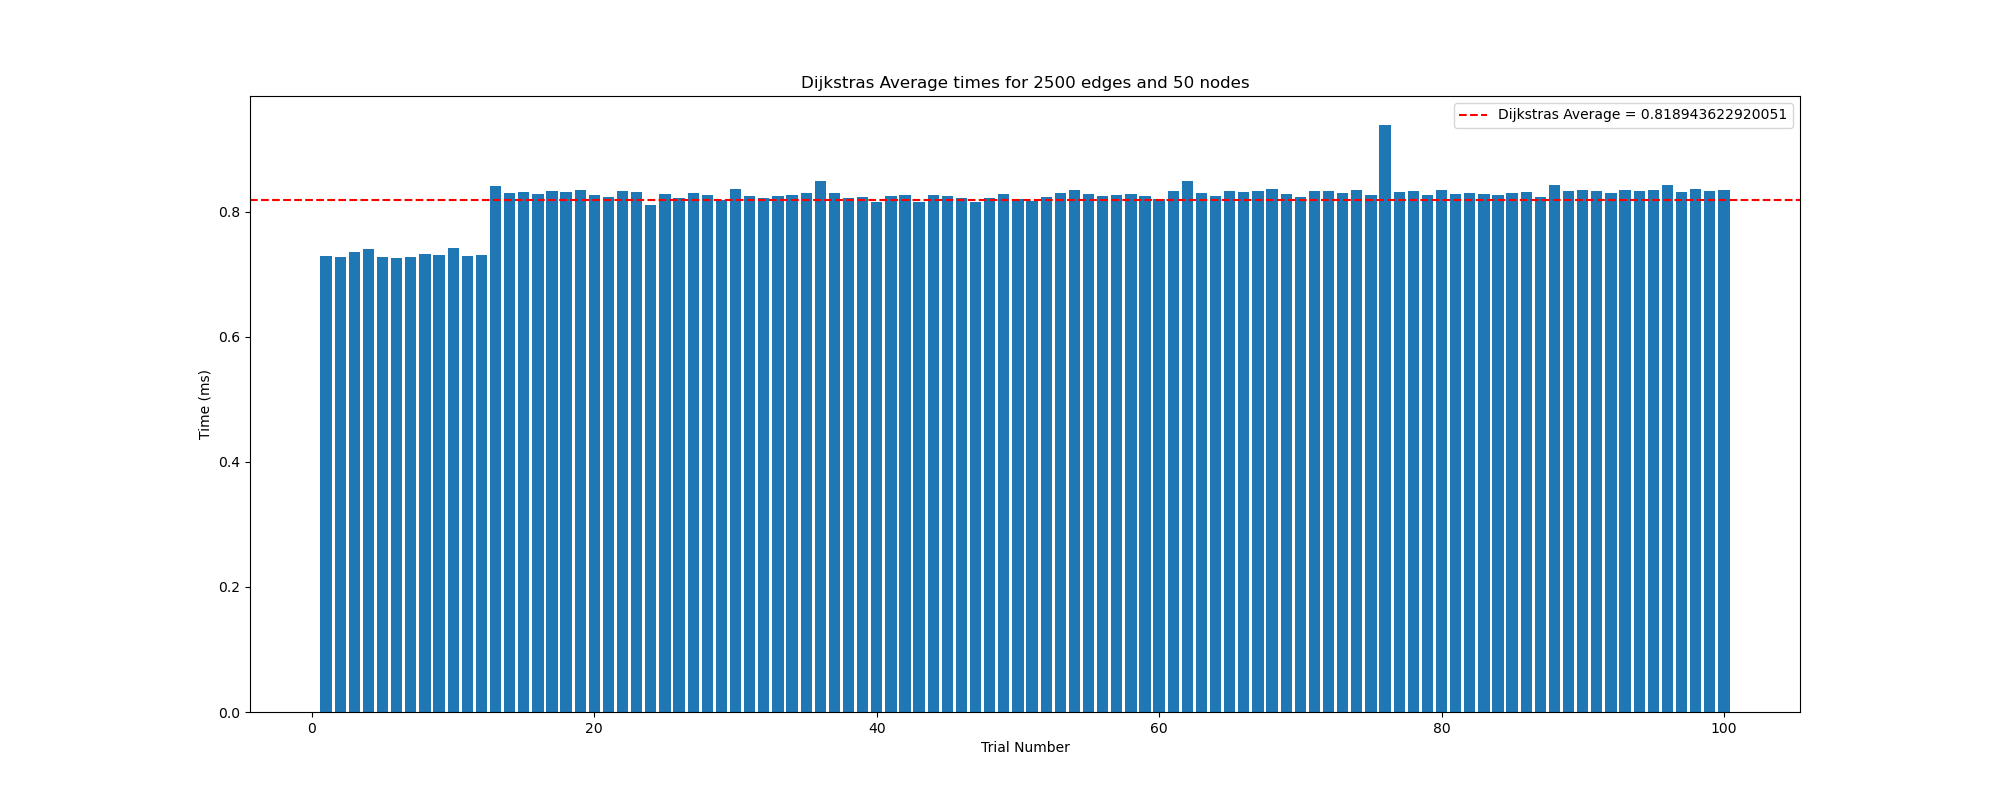
\includegraphics[width=\textwidth]{images/Dijkstras Average times for 2500 edges and 50 nodes.png}
    \caption{Dijkstra's Average times for 2500 edges and 50 nodes}
\end{figure}

\newpage
\section*{Part 3: All-pair shortest path algorithm}
\addcontentsline{toc}{section}{Part 3: All-pair shortest path algorithm}
For this part, I used a modified version of the Floyd-Warshall algorithm that takes a weighted graph, represented by an adjacency list, and converts it into a matrix with the smallest path between all vertex pairs \(u, v\).\newline
\newline
For the second part, we must consider how the complexity of Dijkstra's algorithm and Bellman-Ford would change when running them on dense graphs to find all-pairs shortest paths, which are defined as graphs where \(E \approx V^2\).

\subsection*{Dijkstra's Algorithm}
\addcontentsline{toc}{subsection}{Dijkstra's Algorithm}
We know that Dijkstra's algorithm has a time complexity of \(\Theta(V^2)\). When performing all-pairs shortest paths, we are essentially running Dijkstra's on every single vertex as the source. Since there are \(V\) vertices, the total complexity becomes:
\[
\Theta(V^2) \times V = \Theta(V^3)
\]
However, the drawback of Dijkstra's algorithm is that it does not work on graphs with negative edge weights.

\subsection*{Bellman-Ford Algorithm}
\addcontentsline{toc}{subsection}{Bellman-Ford Algorithm}
We know that Bellman-Ford has a time complexity of \(\Theta(VE)\), which becomes \(\Theta(V^3)\) for dense graphs where \(E \approx V^2\). When performing all-pairs shortest paths, we are running Bellman-Ford on every single vertex as the source. Since there are \(V\) vertices, the total complexity becomes:
\[
\Theta(V^3) \times V = \Theta(V^4)
\]
While this is slower than Dijkstra's, Bellman-Ford is capable of handling negative edge weights and can detect negative cycles.

\subsection*{Choosing an Algorithm} 
\addcontentsline{toc}{subsection}{Choosing an Algorithm}
Since Dijkstra only works on positively weighted graphs and Bellman-Ford is slower, I decided to implement the Floyd-Warshall algorithm, which uses dynamic programming to find the all-pairs shortest paths. It works with both negative and positive edge weights. \newline
\newline
Floyd-Warshall has a time complexity of \(\Theta(V^3)\), making it just as fast as all-pairs Dijkstra’s but more universal due to its ability to handle negative weights.

\subsection*{Conclusion}
\addcontentsline{toc}{subsection}{Conclusion}
Thus, while Dijkstra’s algorithm and Bellman-Ford are useful for single-source shortest path problems, the Floyd-Warshall algorithm is better suited for the all-pairs shortest path problem, especially in dense graphs, as it has a time complexity of \(\Theta(V^3)\) and supports both negative and positive edge weights.

\newpage
\section*{Part 4: A* algorithm}
\addcontentsline{toc}{section}{Part 4: A* algorithm}

\subsection*{Part 4.2}
\addcontentsline{toc}{subsection}{4.2: Comparing A* and Dijkstra's}
\subsubsection*{What issues with Dijkstra's is A* trying to address?}
\addcontentsline{toc}{subsubsection}{What issues with Dijkstra's is A* trying to address?}
The main issue with Dijkstra's algorithm that the A* algorithm tries to address is Dijkstra's lack of
weighting on how close a node is to the target. Dijkstra's picks the node it examines next based on how close 
the source is to the node, but it doesn't take into consideration how close that given node is to the end.
With A* a heuristic function is also taken into consideration which scores each node based on how far it is
perceived to be from the end. This is then taken into account along with the actual distance from the source.
This can lead to faster results when the heuristic is much greater than distance to each node.

\subsubsection*{How would you empirically test Dijkstra’s vs A*?}
\addcontentsline{toc}{subsubsection}{How would you empirically test Dijkstra’s vs A*?}
To test Dijkstra's vs A* I would test based on a few parameters. First I would test them based on a number of
graphs of different numbers of nodes to see how adding more nodes affects the performance of each. I would also
test different levels of density in the graphs to see which one performs on better on sparse and dense graphs.
Finally I would change the weighting of the chosen heuristic function for A* around. I would test scenarios where
the heuristic function is 0, much smaller than the distance, equal to the distance, and much greater than the distance. \\
So in total, my experiment would have the following changing parameters:
\begin{enumerate}
    \item Different amount of nodes: (100, 1000, 10000)
    \item Different graph densities: (V, 2V, V * (V-1)/2)
    \item Different heuristic weightings: (0, much smaller, equal, much greater)
\end{enumerate}
This would given 3 * 3 * 4 = 36 different total testing scenarios. I would then run each of these scenarios for 100 trials,
generating one graph per trial and testing it on both A* and Dijkstra's. I would then graph the results, and keep track of 
the averages.

\subsubsection*{If you generated an arbitrary heuristic function (like randomly generating weights), how
would Dijkstra’s algorithm compare to A*?}
\addcontentsline{toc}{subsubsection}{If you generated an arbitrary heuristic function (like randomly generating weights), how
would Dijkstra’s algorithm compare to A*?}
If you generated the heuristic function randomly, then its performance compared to Dijkstra's would depend on how large the heuristic
values are relative to the real distance of each node from the source. If the heuristic values are sufficiently large 
(much greater than real distance), then this could cause A* to get a wildly wrong answer as it may never examine even close to the 
shortest path. Where as if the heuristic value were sufficiently small (much small than real distance) it would analyze different more
random paths first, leading to a longer runtime than Dijkstra’s, but still end up on the right path. Overall, it would depend on the
magnitude of values in the heuristic function relative to the real distances, but in any case, choosing a random heuristic function
would almost always cause Dijkstra's to perform better by either being faster or by delivering a much better result.

\subsubsection*{What applications would you use A* instead of Dijkstra’s?}
\addcontentsline{toc}{subsubsection}{What applications would you use A* instead of Dijkstra’s?}
Applications where A* is better tend to be ones with a clear and easy to calculate heuristic function. For example, lets say you were
trying to find the shortest path from one city to another through a series of inter-city highways. An easy heuristic function would 
be to real euclidean distance between each city and the destination city, as generally you want to drive towards the city and not away. 
Although this would not exactly match with the real travel time between cities, and may not return the true shortest path if weighted
too heavily. A* is also better in applications where the exact correct answer isn't necessarily needed and a faster answer is
more important. This is because with a good heuristic function that is weighted much more than the real distance, A* is able to find
an answer quickly that is most likely close to the best answer. \\
Thus the applications I would use A* instead of Dijkstra's are those where a good heuristic function is easy to find, and where speed is more important
than path correctness.

\newpage
\section*{Part 5: Compare Shortest Path Algorithms}
\addcontentsline{toc}{section}{Part 5: Compare Shortest Path Algorithms}
\subsection*{Point 1}
\addcontentsline{toc}{subsection}{Point 1}
In our experiment we compared Dijkstra’s against A* using the heuristic of euclidean distance from 
each node to the desired destination. The heuristic was also tested with 5 different multipliers: 0.25, 0.5, 1, 2, and 5.

To compare them visually, we graphed the accuracy and time saved (relative to Dijkstra's) of A* for each level of heuristic.
Accuracy was gauged by dividing the length of the real shortest path (from Dijkstra's) by the length produced by the A* run.
This produced the following graphs:
\begin{figure}[H]
    \centering
    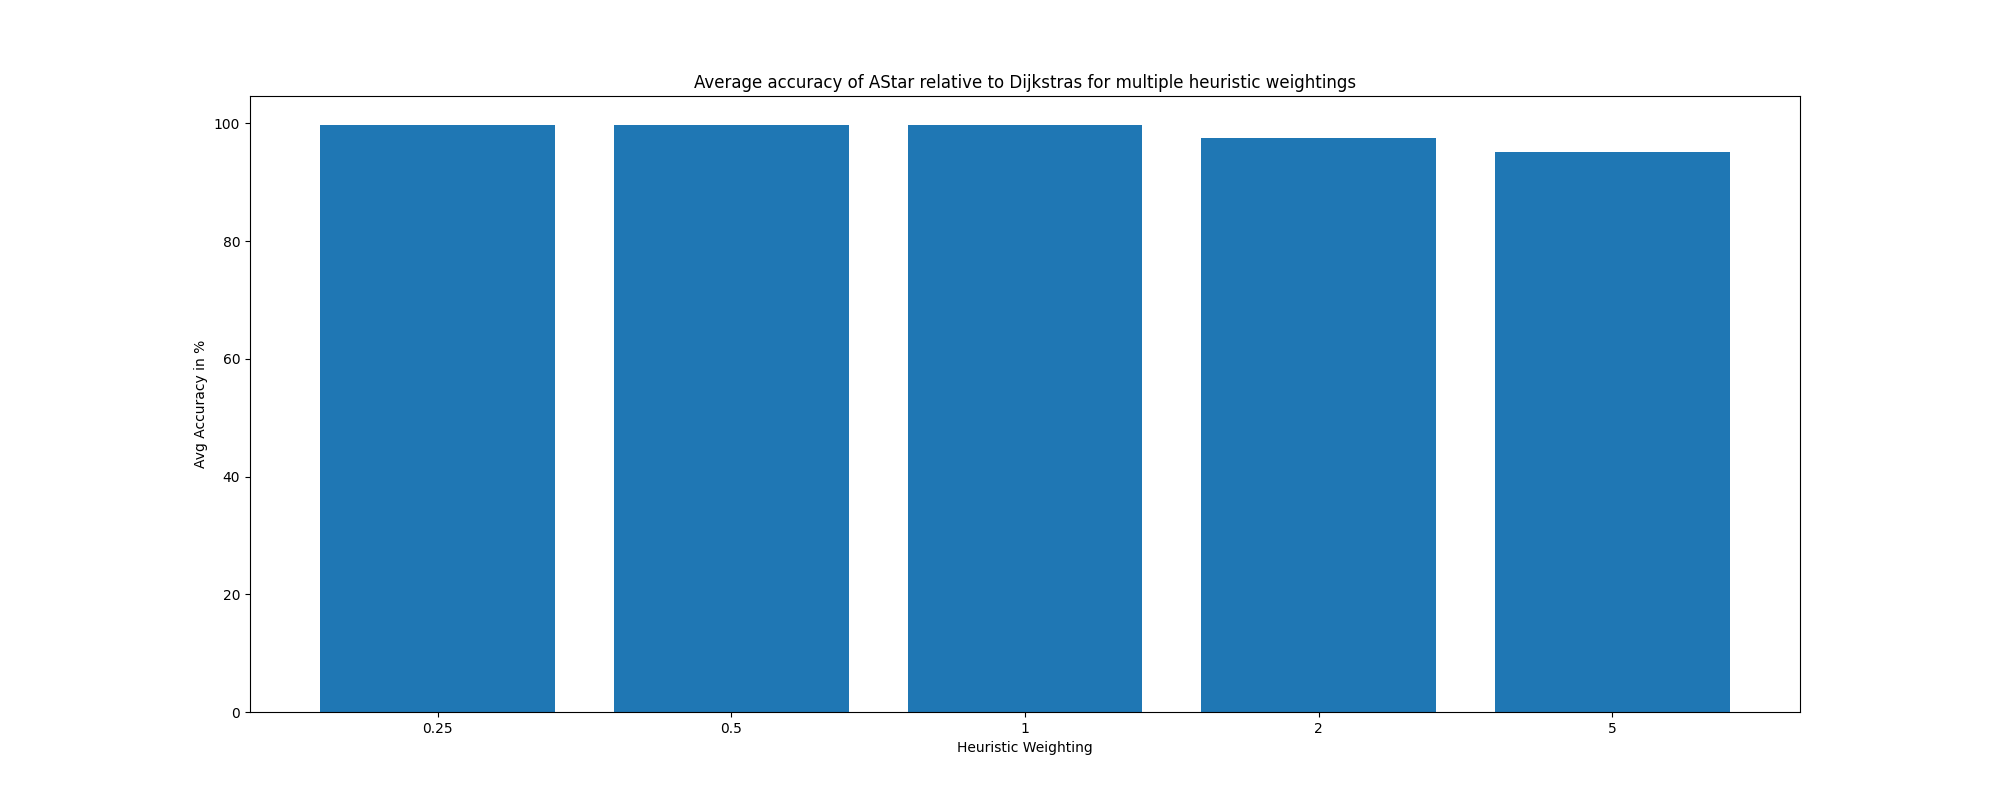
\includegraphics[width=\textwidth]{images/Average accuracy of AStar relative to Dijkstras for multiple heuristic weightings.png}
    \caption{Average accuracy of AStar relative to Dijkstras for multiple heuristic weightings}
\end{figure}

\begin{figure}[H]
    \centering
    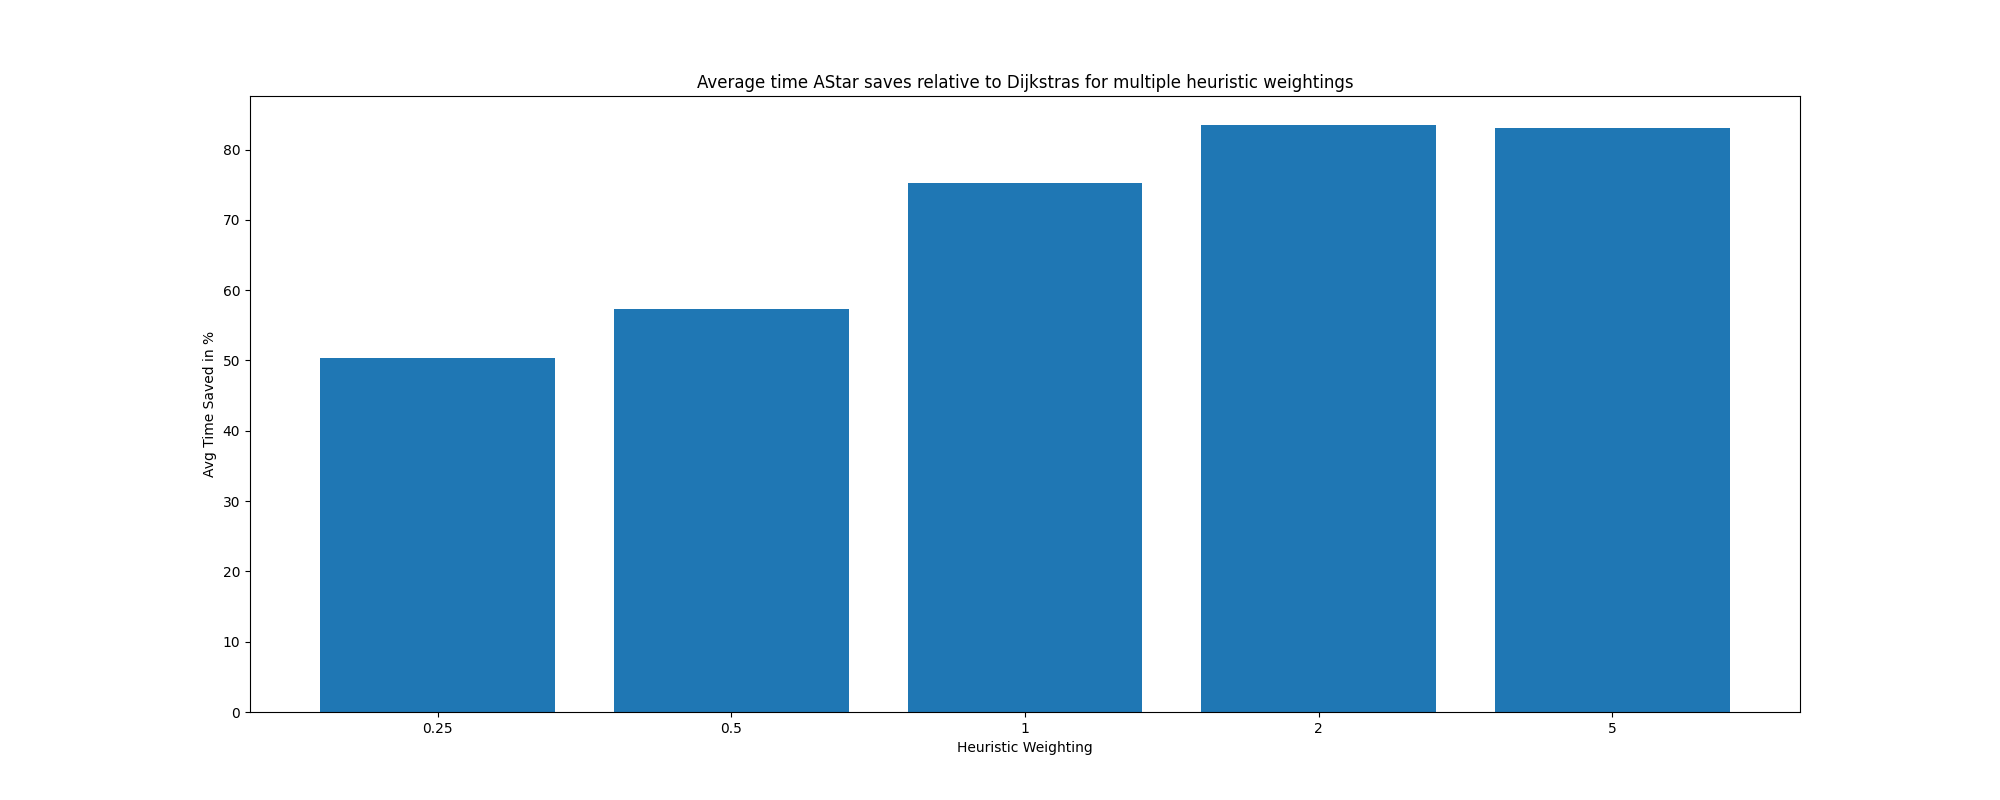
\includegraphics[width=\textwidth]{images/Average time AStar saves relative to Dijkstras for multiple heuristic weightings.png}
    \caption{Average time AStar saves relative to Dijkstras for multiple heuristic weightings}
\end{figure}

From our experiment we saw that even with a heuristic multiplier of just 0.25, A* reduces the runtime of the same search by
an average of 50\% while still maintaining an accuracy of 99.67\%. As the heuristic multiplier increases, this amount of time
saved increases, peaking at 83.45\% when the multiplier is 2. However, as the heuristic multiplier increases

\newpage
\section*{Part 6: Organize your code as per UML diagram}
\addcontentsline{toc}{section}{Part 6: Organize your code as per UML diagram}
Point 1 has nothing to discuss.

\subsection*{Point 2}
\addcontentsline{toc}{subsection}{Point 2}
\textbf{Discuss what design principles and patterns are being used in the diagram.}

There are many design principles and patterns being used in the diagram so I will list them in jot note form:
\begin{itemize}
    \item Inheritance is used in the diagram as the WeightedGraph inherits from Graph and HeuristicGraph inherits from WeightedGraph.
    \item The adapter design pattern is used when implementing the Dijkstra, Bellman\_Ford, and A\_Star as they use previously implemented functions 
          and adapt the input to get the desired output.
    \item Polymorphism is used in the SPAlgorithm class as we can use different algorithms seamlessly via the one "cal\_sp" function.
    \item Encapsulation is used in the HeuristicGraph as it makes the heuristic dictionary private and only shares it through a getter function.
\end{itemize}

\subsection*{Point 3}
\addcontentsline{toc}{subsection}{Point 3}
\textbf{The UML is limited in the sense that graph nodes are represented by the integers. How would you alter the UML diagram to accommodate various needs such as nodes being represented as Strings or carrying more information than their names.? Explain how you would change the design in Figure 2 to be robust to these potential changes.}

In order to allow nodes to carry more information than just their names, we will create a Node class that will store the information for the node, but most importantly, a String for the node's name. This will allow us to have the node be represented via a String while still being able to carry more information than just the name. Following this new class creation, we would need to update the Graph implementations to take in nodes as Nodes instead of integers; this would be simple and require a few name changes and using the name of the node when comparing instead of the object itself, this could be done through a getter function or by accessing the variable directly.

\end{document}
